\documentclass[fr]{../../../../../../eplexam}
\usepackage{tikz}
\usepackage{pgfplots}
\hypertitle{EDPs et analyse complexe}{3}{EPL}{1103}{2021}{Janvier}{All}
{Brieuc Balon}
{Grégoire Winckelmans, Philippe Chatelain et Julien Hendrickx}

\section{Equation des caractéristiques}
On considére l'EDP suivante pour $u(x,y)$ :
\begin{equation*}
    y^{2n-1} \frac{du}{dx} - x^{2n-1} \frac{du}{dy} = \frac{y^{4n-1}}{x^{2n-1}} U
\end{equation*}
avec $n\geq 1$ entier, et U une constante de mêmes unités que u. Le problème de Cauchy est défini avec $\Gamma$ tel que $\left\{
    \begin{array}{ll}
        x(s)=s & \mbox{avec } \ s>0 \\
        y(s)=0
    \end{array}
\right.$ On y prescrit la valeur de la fonction u(s,0)=0.
\begin{enumerate}
    \item Obtenez l'équation des caractéristiques. Esquissez (proprement !) la caractérisitique qui émane d'un s, et ce pour le cas $n>1$ et $n=10$ (Aide : examinez le point tel que x=y, avec l'information que $2^{\frac{9}{20}} \approx 0.966\sqrt{2}$). Quelle forme particulière avons-nous pour la caractéristique lorsque $n \rightarrow +\infty$.
    \item Obtenez la solution détaillée de $u(x,y)$.
    
\end{enumerate}
\begin{solution}
\begin{enumerate}
    \item En écrivant l'équation des caractéristiques :
\begin{align*}
    \textcolor{red}{\int_{0}^{y}}y^{2n-1}\textcolor{red}{dy} &=-\textcolor{red}{\int_{s}^{x}}x^{2n-1} \textcolor{red}{dx} \\
    \Leftrightarrow \frac{y^{2n}}{2n} &= -\left[ \frac{x^{2n}}{2n} \right]_{s}^{x}\\
     \Leftrightarrow \frac{s^{2n}}{2n} &= \frac{y^{2n}}{2n}+\frac{x^{2n}}{2n} \\
     \Leftrightarrow s &=\sqrt[2n]{x^{2n}+y^{2n}}
\end{align*}
Pour $n=1$ on a $x^2+y^2=s^2$. La caractéristique qui émane de s est un cercle de rayon s 
\begin{center}
\begin{tikzpicture}
  \begin{axis}[
    axis lines = left,
    xlabel = $\frac{x}{L}$,
    ylabel = {$\frac{y}{L}$},
]
\addplot[mark=none, red] coordinates {(0,0) (2,0)};
\addplot [
    domain=0:2, 
    samples=100, 
    color=blue,
]
{(2^2 - x^2)^(1/2) };

d
\addplot [
    domain=0:1, 
    samples=100, 
    color=blue,
    ]
    {(1^2 - x^2)^(1/2)};

\addplot [
    domain=0:1.5, 
    samples=100, 
    color=blue,
    ]
    {(1.5^2 - x^2)^(1/2)};
\end{axis}
\end{tikzpicture}
\end{center}
Traçons pour $n=3$ 
\begin{center}
\begin{tikzpicture}
  \begin{axis}[
    axis lines = left,
    xlabel = $\frac{x}{L}$,
    ylabel = {$\frac{y}{L}$},
]
\addplot[mark=none, red] coordinates {(0,0) (2,0)};
\addplot [
    domain=0:2, 
    samples=900, 
    color=blue,
]
{(2^6 - x^6)^(1/6) };

d
\addplot [
    domain=0:1, 
    samples=900, 
    color=blue,
    ]
    {(1^6 - x^6)^(1/6)};

\addplot [
    domain=0:1.5, 
    samples=900, 
    color=blue,
    ]
    {(1.5^6 - x^6)^(1/6)};
\end{axis}
\end{tikzpicture}
\end{center}

Traçons pour $n=10$ :
\begin{center}
\begin{tikzpicture}
  \begin{axis}[
    axis lines = left,
    xlabel = $\frac{x}{L}$,
    ylabel = {$\frac{y}{L}$},
]

\addplot [
    domain=0:2, 
    samples=1200, 
    color=blue,
]
{(2^20 - x^20)^(1/20) };


\addplot [
    domain=0:1, 
    samples=1200, 
    color=blue,
    ]
    {(1^20 - x^20)^(1/20)};

\addplot [
    domain=0:1.5, 
    samples=1200, 
    color=blue,
    ]
    {(1.5^20 - x^20)^(1/20)};
    \addplot[mark=none, red] coordinates {(0,0) (2,0)};
\end{axis}
\end{tikzpicture}
\end{center}
Pour $n\rightarrow \infty$ nous aurons des caractéristiques rectangulaires :
\begin{center}
\begin{tikzpicture}
  \begin{axis}[
    axis lines = left,
    xlabel = $\frac{x}{L}$,
    ylabel = {$\frac{y}{L}$},
]
\addplot[mark=none, red] coordinates {(0,0) (2,0)};
\addplot[mark=none, blue] coordinates {(0,1) (1,1)};
\addplot[mark=none, blue] coordinates {(0,2) (2,2)};
\addplot[mark=none, blue] coordinates {(1,0) (1,1)};
\addplot[mark=none, blue] coordinates {(1.5,0) (1.5,1.5)};
\addplot[mark=none, blue] coordinates {(2,0) (2,2)};
\addplot[mark=none, blue] coordinates {(0,1.5) (1.5,1.5)};
\end{axis}
\end{tikzpicture}
\end{center}
\item Le long de la caractéristique qui émane de $s$ nous avons : 
\begin{center}
\begin{equation*}
    P du = R dx ~~~~~~~~Q du = R dy 
\end{equation*}
\end{center}
Prenons la première :
\begin{equation*}
    y^{2n-1} du = \frac{y^{4n-1}}{x^{2n+1}}Udx \Leftrightarrow du = \frac{y^{2n}}{x^{2n+1}}Udx
\end{equation*}
Comme $y^{2n} = s^{2n}- x^{2n}$
\begin{align*}
    du &= U \frac{(s^{2n}-x^{2n}}{x^{2n+1}}dx\\
    &= U \left[s^{2n}\frac{dx}{x^{2n+1}}- \frac{dx}{x} \right]\\
    \Rightarrow \int_{u(s,0)}^{u(x,y)}du &= U \left[ s^{2n} \int_s^x\frac{dx}{x^{2n+1}} - \int_s^x \frac{dx}{x}\right]\\
   \Leftrightarrow u(x,y) - \overbrace{u(s,0)}^{=0} &= U \left[ s^{2n} -\frac{1}{2n}\left(\frac{1}{x^{2n}}-\frac{1}{s^{2n}}\right)-\ln\left(\frac{x}{s}\right)\right]\\
   \Leftrightarrow u(x,y) &= U \left[ \frac{1}{2n} \left(1 - \frac{s^{2n}}{x^{2n}}\right) + \ln\left(\frac{s}{x}\right)\right]
\end{align*}
Comme $s^{2n}= x^{2n}+y^{2n} \Leftrightarrow \frac{s^{2n}}{x^{2n}} = 1 + \frac{y^{2n}}{x^{2n}}$
\begin{equation*}
    \Rightarrow u(x,y) = U \left[ \ln\left(\frac{s}{x}\right)-\frac{1}{2n}\left(\frac{y}{x}\right)^{2n}\right]
\end{equation*}
\end{enumerate}
\end{solution}


\section{Titre de la seconde question}

On considère le champ de température u dans un disque $r \leq a$. On impose une première température sur sa circonférence $f_1(\theta)$. On laisse une temps très long (= infini) au champ de température pour s'établir comme $u_1(r,\theta)$ dans le disque.
\begin{enumerate}
    \item Quelle équation satisfait $u_1$ ? Justifiez brievement.
    \item On change la température sur la circonférence $f_2(\theta)$ et à nouveau on laisse un temps très long (= infini) au champ de température pour s'établir comme $u_2(r,\theta)$. En exploitant vos connaissances sur la réponse précédente et sans résoudre les champs $u_1$ et $u_2$ déterminez la quantité d'énergie à extraire pour passer de $u_1$ à $u_2$. 
    \begin{equation*}
        \Delta E = c \int_{0}^{2\pi} \int_{0}^{a} u_2 r \, \mathrm{d}r\mathrm{d}\theta - c \int_{0}^{2\pi} \int_{0}^{a} u_1 r \, \mathrm{d}r\mathrm{d}\theta
    \end{equation*} où c est la chaleur spécifique du matériau du disque (constant ici). On donne les expressions suivantes pour conditions aux frontières
    \begin{equation*}
    \begin{cases}
     f_1(\theta) = A + B \cos^2(\theta)\sin(\theta) \\ f_2(\theta) = C + D \sin^3(\theta)\cos(\theta)
    \end{cases}    
    \end{equation*}
    \noindent Justifier votre approche. Cet exercice n'est que très modérément calculatoire. Rappel : $\int f(g(x))g'(x) dx = \int f(g)dg$.
    
\end{enumerate}
\begin{solution}
    \begin{enumerate}
        \item Le problème original est un problème de diffusion régi par l'équation parabolique $\frac{\partial u}{\partial t} = D \grad^2u$. On laisse un temps infini pour atteindre la solution de régime de cette équation. Cela correspond à $\frac{\partial u}{\partial t}=0$. Cela signifie que $u_1$ respectera l'équation de Laplace $\grad^2 u_1 =0$
        \item $u_2$, comme $u_1$, est une solution de régime de $\frac{\partial u}{\partial t} = D \grad^2u$. Elles sont donc solution de l'équation de Laplace $\grad^2u_2 =0$. On veut calculer l'intégrale de chacune des solutions sur un cercle. Pour ce faire nous utiliserons le théorème de la moyenne. 
        \begin{equation*}
        \underbrace{u_*(0,\theta)}_{\text{Valeur au centre}} = \underbrace{\frac{1}{2\pi a}\int_0^{2\pi} u_*(a,\theta) a d\theta}_{\text{Moyenne sur la circonférence}}= \underbrace{\frac{1}{\pi a^2}\int_0^a\int_0^{2\pi}u_*(r,\theta)r d\theta dr}_{\text{Moyenne sur l'aire}}
        \end{equation*}
        Avec $*$ qui correspond à 1 ou 2. On peut donc écrire :
        \begin{equation*}           
        \int_0^a\int_0^{2\pi}u_*(r,\theta)r d\theta dr = \frac{a^2}{2}\int_0^{2\pi}u_*d\theta
        \end{equation*}
        \begin{align*}
            \Delta E &= c \frac{a^2}{2}\left(\int_0^{2\pi}u_2d\theta - \int_0^{2\pi}u_1d\theta\right)\\
            \Rightarrow &\int_0^{2\pi} f_1(\theta) d\theta = \int_0^{2\pi} (A+B \underbrace{\cos^2(\theta) \sin(\theta)}_{g(\theta) = \cos(\theta)\atop g'(\theta) = - \sin(\theta)})d\theta = 2\pi A + B\left[ -\frac{\cos^3(\theta)}{3}\right]_{0}^{2\pi}= 2\pi A\\
            \Rightarrow &\int_0^{2\pi} f_2(\theta) d\theta = \int_0^{2\pi} (C+D \underbrace{\sin^3(\theta) \cos(\theta)}_{g(\theta) = \sin(\theta)\atop g'(\theta) = \cos(\theta)})d\theta = 2\pi C + D\left[ \frac{\sin^4(\theta)}{4}\right]_{0}^{2\pi}= 2\pi C\\
            &\Rightarrow \Delta E = \pi c a^2 (C-A)
        \end{align*}
    \end{enumerate}
\end{solution}
\section{Méthode de séparation des variables}
On considère l'EDP suivante pour $u(r,\theta)$ :
\begin{equation*}
    \grad^2 u = \frac{\partial^2 u}{\partial r^2} + \frac{1}{r}\frac{\partial u}{\partial r}+\frac{1}{r^2}\frac{\partial^2u}{\partial\theta^2}=0
\end{equation*}
et ce à l'intérieur d'un secteur de disque de rayon et d'angle d'ouverture $\beta = \frac{2\pi}{3}$. On impose que $u(a,\theta) = U(\frac{\theta}{\beta})^2$ avec U constant, tel que $\frac{\partial u}{\partial\theta}(r,0)=0$ et que $u(r,\beta) = U (\frac{r}{a})^3$. Obtenez la solution en utilisant une superposition ($u=u_1+u_2$) et la méthode de séparation de variable. (Aide : utilisez la fonction $U(\frac{r}{a})^n \cos(n\theta)$ avec n entier dans votre décomposition. Elle satisfait l'EDP.) Définissez clairement les deux sous problèmes avec esquisses. A la fin : écrire clairement les intégrales à évaluer pour obtenir les coefficients du développement en série, mais ne pas les évaluer. Rappel : l'EDO $r'R''+rR'-k^2R=0$ a comme solution $R(r) = C(\frac{r}{L})^k+D(\frac{r}{L})^{-k}$ où L est une longueur caractéristique du problème.
\begin{solution}
En traçant les conditions aux limites
\begin{center}
    \begin{tikzpicture}
    \begin{scope}[thick,font=\scriptsize]
    
    \draw [->] (0,0) -- (5,0) node [below]  {$r$};
    \draw [->] (0,0) -- (0,4) node [below left] {$\Theta$};


    \draw (3.5,3pt) -- (3.5,-3pt)   node [below] {$a$};
    \draw (3pt,2.5) -- (-3pt,2.5)   node [left] {$\beta$};
    \draw [->,red] (0,1.5) -- (-0.5,1.5) node [left,red]  {u régulière};`
    \draw [->,red] (1.5,0) -- (1.5,-0.5) node [below,red]  {$\frac{\partial u}{\partial\theta}(r,0)=0$};
    \draw [->,red] (3.5,1.5) -- (4,1.5) node [right,red]  {$u(a,\theta) = U(\frac{\theta}{\beta})^2$};
    \draw [->,red] (1.5,2.5) -- (1.5,3) node [above,red]  {$u(r,\beta) = U (\frac{r}{a})^3$};
    \draw (0,0) -- (0,2.5)--(3.5,2.5) -- (3.5,0) -- (0,0)[red];

    \end{scope}
    \end{tikzpicture}
    
    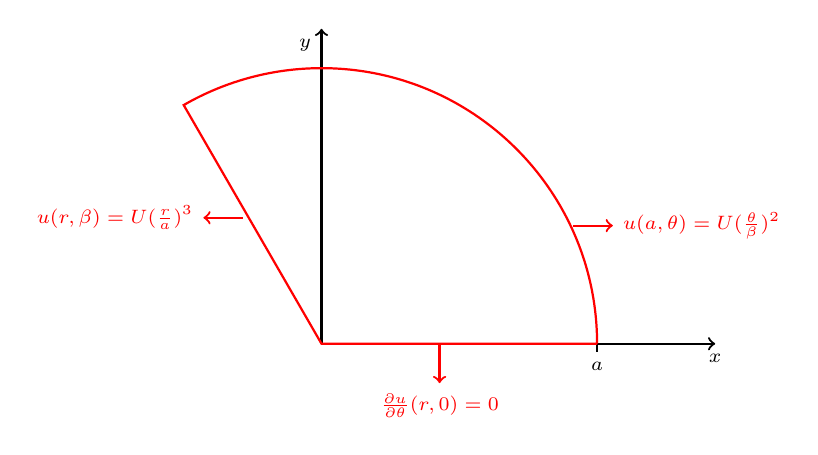
\begin{tikzpicture}
    \begin{scope}[thick,font=\scriptsize]
    
    \draw [->] (0,0) -- (5,0) node [below]  {$x$};
    \draw [->] (0,0) -- (0,4) node [below left] {$y$};


    \draw (3.5,3pt) -- (3.5,-3pt)   node [below] {$a$};
    \draw (3.5,0) arc(0:120:3.5)[red] -- (0,0)--(3.5,0)[red];
    
    \draw [->,red] (1.5,0) -- (1.5,-0.5) node [below,red]  {$\frac{\partial u}{\partial\theta}(r,0)=0$};
    \draw [->,red] (3.2,1.5) -- (3.7,1.5) node [right,red]  {$u(a,\theta) = U(\frac{\theta}{\beta})^2$};
    \draw [->,red] (-1,1.6) -- (-1.5,1.6) node [left,red]  {$u(r,\beta) = U (\frac{r}{a})^3$};
   
    

    \end{scope}
    \end{tikzpicture}
    
\end{center}
Comme il n'y a pas deux conditions aux limites homogènes dans la direction de $\theta$ on divise le problème en deux sous-problèmes. Pour se faire, on utilise l'aide, qui satisfait les conditions aux limites, pour déterminer celles de la superposition. 

\begin{align*}
    &U_1 = U\left(\frac{r}{a}\right)^n\cos(n\theta)\\
    &\Rightarrow \frac{\partial U_1}{\partial\theta}(r,0)=- U \left(\frac{r}{a}\right)^n n \sin(n\cdot 0) = 0\\
    &\Rightarrow U_1(r,\frac{2\pi}{3}) = U\left(\frac{r}{a}\right)^n\cos\left(n\frac{2\pi}{3}\right) = U \left(\frac{r}{a}\right)^3
\end{align*}
On remarque que pour respecter la deuxième condition, il faut que $n=3$. Donc 
\begin{equation*}
    U_1(r,\theta)= U\left(\frac{r}{a}\right)^3\cos(3\theta)
\end{equation*}
Nous pouvons écrire la superposition en prenant les sous-problèmes suivant :
\begin{center}
    
    
    \begin{tikzpicture}
    \begin{scope}[thick,font=\scriptsize]
    
    \draw [->] (0,0) -- (5,0) node [below]  {$x$};
    \draw [->] (0,0) -- (0,4) node [below left] {$y$};


    \draw (3.5,3pt) -- (3.5,-3pt)   node [below] {$a$};
    \draw (3.5,0) arc(0:120:3.5)[red] -- (0,0)--(3.5,0)[red];
    
    \draw [->,red] (1.5,0) -- (1.5,-0.5) node [below,red]  {$\frac{\partial u_1}{\partial\theta}(r,0)=0$};
    \draw [->,red] (3.2,1.5) -- (3.7,1.5) node [right,red]  {$u_1(a,\theta) = U \cos(3\theta)$};
    \draw [->,red] (-1,1.6) -- (-1.5,1.6) node [left,red]  {$u_1(r,\beta) = U (\frac{r}{a})^3$};
   
    

    \end{scope}
    \end{tikzpicture}
    


    \begin{tikzpicture}
    \begin{scope}[thick,font=\scriptsize]
    
    \draw [->] (0,0) -- (5,0) node [below]  {$x$};
    \draw [->] (0,0) -- (0,4) node [below left] {$y$};


    \draw (3.5,3pt) -- (3.5,-3pt)   node [below] {$a$};
    \draw (3.5,0) arc(0:120:3.5)[red] -- (0,0)--(3.5,0)[red];
    
    \draw [->,red] (1.5,0) -- (1.5,-0.5) node [below,red]  {$\frac{\partial u_2}{\partial\theta}(r,0)=0$};
    \draw [->,red] (3.2,1.5) -- (3.7,1.5) node [right,red]  {$u_2(a,\theta) = U(\frac{\theta}{\beta})^2 - U \cos(3\theta)$};
    \draw [->,red] (-1,1.6) -- (-1.5,1.6) node [left,red]  {$u_2(r,\beta) = 0$};
   
    \end{scope}
    \end{tikzpicture}
    
\end{center}
On remarque que la somme des CL des 2 sous-problèmes donne bien celles du problème initial.\\
    
\noindent Par la méthode de séparation des variables, on pose $u(r,\theta) = R(r)\Theta(\theta)$. L'EDP prend la forme : 
\begin{align*}
    R''\Theta + \frac{1}{r}R'\Theta + \frac{1}{r^2}R\Theta'' &=0\\
    r^2 \frac{R''}{R} + r \frac{R'}{R} + \frac{\Theta''}{\Theta} &= 0\\
    \frac{r^2R''+r R'}{R} = -\frac{\Theta''}{\Theta} &=\lambda
\end{align*}
Nous avons déjà déterminer $u_1$ et donc la condition pour $\lambda =0$.\\

\noindent Nous avons pour $u_2$ que $\lambda >0 \rightarrow \lambda =k^2$ car nous avons des CL homogènes en $\theta$.
\begin{align*}
    \Theta'' + k^2 \Theta &=0 \\
    \Rightarrow \Theta(\theta) &= A \cos(k\theta) + B \sin(k\theta)
\end{align*}
Avec les différentes CL : 
\begin{align*}
    \frac{\partial u_2}{\partial\theta}(r,0)=0 &\Rightarrow \Theta'(0) =0\\
    & - Ak \sin(0) + Bk \cos(0) = 0\\
    &\Rightarrow B =0\\
    \\
    u_2(r,\beta) =0 &\Rightarrow A \cos(k\beta) = 0\\
    &\Leftrightarrow k\beta = \frac{\pi}{2},\frac{3\pi}{2},\frac{5\pi}{2},...\\
    &\Leftrightarrow k\beta = (2n-1)\frac{\pi}{2}~~n =1,2,...
\end{align*}
Nous obtenons :
\begin{equation*}
    \Theta_n(\theta) = A_n \cos(k_n\theta) 
\end{equation*}
Pour $R(r)$ grâce au rappel sur l'EDO d'Euler, nous trouvons
\begin{align*}
    &r^2R'' + rR'-k^2 R = 0\\
    &\Leftrightarrow R(r) = C\left(\frac{r}{a}\right)^k + D \left(\frac{r}{a}\right)^{-k}
\end{align*}
Pour que la solution soit régulière en $r=0$ il faut que $D=0$. Nous trouvons alors:
\begin{equation*}
    R_n(r)= C_n \left(\frac{r}{a}\right)^{k_n}
\end{equation*}
En mettant tout ensemble : 
\begin{align*}
    u_n(r,\theta) &= R_n(r) \Theta_n(\theta) = \underbrace{A_nC_n}_{\Tilde{A_n}}\left(\frac{r}{a}\right)^{k_n}\cos(k_n\theta)\\
    \Rightarrow u_2(r,\theta) &=  \sum_{n=1}^\infty \Tilde{A_n}\left(\frac{r}{a}\right)^{k_n}\cos(k_n\theta)
\end{align*}
Avec les conditions aux limites :
\begin{equation*}
    u_2(a,\theta) = U \left(\left(\frac{\theta}{\beta}\right)^2-\cos(3\theta)\right) = \sum_{n=1}^\infty \Tilde{A_n}\cos(k_n\theta)
\end{equation*}
Par orthogonalité des fonctions propres
\begin{align*}
    \Tilde{A_n}\textcolor{red}{\int_0^\beta}\cos(k_n\theta)\textcolor{red}{\cos(k_n\theta) d\theta} &= U \textcolor{red}{\int_0^\beta} \left(\left(\frac{\theta}{\beta}\right)^2-\cos(3\theta)\right)\textcolor{red}{\cos(k_n\theta)d\theta}\\
    \Tilde{A_n} \underbrace{\int_0^\beta \cos^2(k_n\theta)d\theta}_{=\frac{\beta}{2}} &= U \int_0^\beta \left(\left(\frac{\theta}{\beta}\right)^2-\cos(3\theta)\right) \cos(k_n\theta) d\theta\\
    &=U \underbrace{\int_0^\beta \left(\frac{\theta}{\beta}\right)^2\cos(k_n\theta)d\theta}_{I_1} - U \underbrace{\int_0^\beta \cos(3\theta)\cos(k_n\theta)d\theta}_{I_2}
\end{align*}
\begin{align*}
    I_1 &= \int_0^\beta \left(\frac{\theta}{\beta}\right)^2\cos(k_n\theta)d\theta \\&= \frac{(\overbrace{k_{n}^2 \beta^2}^{\left((2n-1)\frac{\pi}{2}\right)^2}-2)\overbrace{\sin(\beta k_n)}^{(-1)^{n+1}}+2k_n\beta\overbrace{\cos(k_n\beta)}^{0}}{\beta^2k_{n}^3}\\
    &= \frac{\overbrace{(\left((2n-1)\frac{\pi}{2}\right)^2-2)}^{\alpha}(-1)^{n+1}}{\beta^2k_{n}^3}= \frac{\alpha(-1)^{n+1}}{\beta^2k_{n}^3}\\
    \\
    I_2 &= \int_0^\beta \cos(3\theta)\cos(k_n\theta)d\theta\\
    &=\frac{\sin\left(\beta\left(k_n+3\right)\right)}{2\left(k_n+3\right)}+\frac{\sin\left(\beta\left(k_n-3\right)\right)}{2\left(k_n-3\right)}
\end{align*}
Il ne l'était pas demandé mais
\begin{equation*}
    \Tilde{A_n}= \frac{2U}{\beta}(I_1-I_2)
\end{equation*}
\end{solution}

\section{Intégrale complexe}
On souhaite calculer l'intégrale suivante : 
\begin{equation*}
    I = \int_{0}^{\infty} \frac{1}{(x^4+1)(x^2+1)^2}, \mathrm{d}x
\end{equation*}
\begin{enumerate}
    \item Exprimez la valeur de I en fonction des résidus, que vous ne calculez pas encore.
    \item Calculez les résidus utiles en 4.1 et donnez la valeur explicite pour l'intégrale I.
\end{enumerate}
\begin{solution}
\begin{enumerate}
    \item Prenons une fonction f telle que $f(z) = \frac{1}{(z^4+1)(z^2+1)^2}$. Il faut trouver son domaine de définition:
    \begin{equation*}
        x^4+1=0 \Leftrightarrow x^4 = -1 \Leftrightarrow x^4 = e^{-i\pi + 2k\pi i} \Leftrightarrow x = e^{-\frac{\pi}{4}+\frac{k\pi}{2}}
        \end{equation*}
    En ajoutant les racines du polynôme $x^2+1$ qui seront des pôles de second ordre. Nous obtenons avec $R>1$ : 
    \begin{equation*}
        f : \mathbb{C}  \textbackslash \left\{ e^{\pm \frac{i\pi}{4}}, e^{\pm \frac{3i\pi}{4}}, \pm i \right\} \rightarrow \mathbb{C} : z \rightarrow \frac{1}{(z^4+1)(z^2+1)^2}
    \end{equation*}
\end{enumerate}
\begin{center}

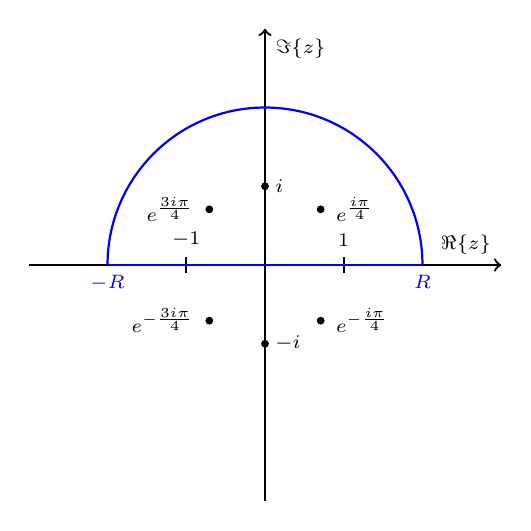
\begin{tikzpicture}
    \begin{scope}[thick,font=\scriptsize]
    % Axes:
    % Are simply drawn using line with the `->` option to make them arrows:
    % The main labels of the axes can be places using `node`s:
    \draw [->] (-3,0) -- (3,0) node [above left]  {$\Re\{z\}$};
    \draw [->] (0,-3) -- (0,3) node [below right] {$\Im\{z\}$};

    % Axes labels:
    % Are drawn using small lines and labeled with `node`s. The placement can be set using options
    
    % If you only want a single label per axis side:
    \draw (1,-3pt) -- (1,3pt)   node [above] {$1$};
    \draw (-1,-3pt) -- (-1,3pt) node [above] {$-1$};
    \draw (0,1)  node [right] {$i$};
    \draw (0,-1) node [right] {$-i$};
    
    \draw (-0.707, -0.707) node[circle,fill,inner sep=1pt,label=left:$e^{-\frac{3i\pi}{4}}$]{};
    \draw (-0.707, 0.707) node[circle,fill,inner sep=1pt,label=left:$e^{\frac{3i\pi}{4}}$]{};
    \draw (0.707, 0.707) node[circle,fill,inner sep=1pt,label=right:$e^{\frac{i\pi}{4}}$]{};
    \draw (0.707, -0.707) node[circle,fill,inner sep=1pt,label=right:$e^{-\frac{i\pi}{4}}$]{};
    \draw (0, -1) node[circle,fill,inner sep=1pt]{};
    \draw (0, 1) node[circle,fill,inner sep=1pt]{};
    \draw (-2,0) node [below, blue] {$-R$};
    \draw (2,0) node [below, blue] {$R$};
    \draw [blue](-2,0) -- (2,0) ;
    \draw (2,0) arc(0:180:2)[blue];
    \end{scope}
    % The circle is drawn with `(x,y) circle (radius)`
    % You can draw the outer border and fill the inner area differently.
    % Here I use gray, semitransparent filling to not cover the axes below the circle
    %\path [draw=none,fill=gray,semitransparent] (+1,-1) circle (3);
    % Place the equation into the circle:
    %\node [below right,gray] at (+1,-1) {$|z-1+i| \leq 3$};
\end{tikzpicture}
\end{center}
Nous avons choisi un contour en demi cercle étant donné que la fonction est paire $f(x) = f(-x)$
\begin{equation*}
    \oint_{\gamma R} f(z) \,dz = \int_{-R}^{R} f(x) \, dx + \int_{0}^{\pi} f(Re^{i\theta})Ri e^{i\theta} \, d\theta = 2\pi i [res(f,e^{\frac{3i\pi}{4}}) + res(f,e^{\frac{i\pi}{4}})+ res(f,i)]
\end{equation*}
On peut démontrer que l'intégrale sur l'arc tend vers 0 : 
\begin{align*}
    |\int_{0}^{\pi} f(Re^{i\theta})Ri e^{i\theta} \, d\theta| &\leq \int_{0}^{\pi} |f(Re^{i\theta})| |Ri| |e^{i\theta}| \, d\theta \\ 
    &= R \int_{0}^{\pi} |\frac{1}{(R^4 e^{4i \theta}+1)(R^2 e^{2i\theta}+1)^2}| \, d\theta \\
    &\leq R \int_{0}^{\pi}\frac{1}{(R^4+1)(R^2+1)^2} \, d\theta \\
    &= \frac{R \pi}{(R^4+1)(R^2+1)^2} \\
    &= 0 ~\mbox{si}~R\rightarrow\infty
\end{align*}
Comme la fonction est paire : 
\begin{equation*}
    \lim_{R\to\infty}\oint_{\gamma R} f(z) \,dz = \int_{-\infty}^{\infty} f(x) \, dx + \lim_{R\to\infty} \int_{0}^{\pi} f(Re^{i\theta})Ri e^{i\theta} \, d\theta = 2 \int_{0}^{\infty} \frac{1}{(x^4+1)(x^2+1)^2} \, dx +0
\end{equation*}
\begin{equation*}
    \Rightarrow \int_{0}^{\infty} \frac{1}{(x^4+1)(x^2+1)^2} \, dx = \pi i [res(f,e^{\frac{3i\pi}{4}}) + res(f,e^{\frac{i\pi}{4}})+ res(f,i)]
\end{equation*}
\item Les résidus peuvent être calculés facilement lorsqu'ils sont d'ordre 1 ($res(f,a) = \frac{P(a)}{Q'(a)}$ si $f = \frac{P}{Q}$ avec P et Q des polynômes).
\begin{equation*}
    res(f,e^{\frac{3i\pi}{4}}) = \frac{1}{[(x^4+1)(x^2+1)^2]'\Big|_{x=e^{\frac{3i\pi}{4}}}} = \frac{1}{4\sqrt{2}(1-i)}
\end{equation*}
\begin{equation*}
    res(f,e^{\frac{i\pi}{4}}) = \frac{1}{[(x^4+1)(x^2+1)^2]'\Big|_{x=e^{\frac{i\pi}{4}}}} = -\frac{1}{4\sqrt{2}(1+i)}
\end{equation*}
Le pôle en $i$ est un pôle d'ordre 2 nous ne pouvons pas utiliser la formule simplifiée. Il faut utiliser $res(f,a) = \lim_{z\to a} \frac{\partial^{n-1} }{\partial z^{n-1}} ((z-a)^n f(z))$ pour un pôle d'ordre n.
\begin{equation*}
    res(f,i) = \lim_{z\to i} \frac{\partial }{\partial z} ((z-i)^2\frac{1}{(z^4+1)(z^2+1)^2}) = -\frac{3i}{8}
\end{equation*}
\begin{equation*}
    \int_{0}^{\infty} \frac{1}{(x^4+1)(x^2+1)^2} \, dx = \pi i [\frac{1}{4\sqrt{2}(1-i)}  -\frac{1}{4\sqrt{2}(1+i)} -\frac{3i}{8}] = \pi i \cdot \frac{-3+\sqrt{2}}{8}i = \pi\frac{3-\sqrt{2}}{8} \simeq 0.6227
\end{equation*}

\end{solution}

\section{Démonstration théorème fondamental de l'algèbre}
Soit $f : \mathbb{C} \rightarrow \mathbb{C}$ une fonction holomorphe et soit $n \in \mathbb{N}$. Démontrez que s'il existe des réels $M\geq 0$ et $r>0$ tels que pour tout $z\in \mathbb{C}$, $|z|\geq r$ implique $|f(z)| \leq M |z|^n$, alors f est polynomiale de degré au plus n. 

Bonus : Que pouvez-vous affirmer si $|f(z)| \leq M |z|^n$ est remplacé par $f(z) \leq M|z|^\frac{3}{2}$ ? 
\begin{solution}
Comme f est holomorphe, on sait que pour n'importe quel réel $R>|z|$:
\begin{equation*}
    \forall z \in \mathbb{C} : ~ f(z) = \sum_{k=0}^{\infty} a_k z^k  ~~~~~\mbox{avec} ~~~~~ a_k = \frac{1}{2\pi i}\int_{\partial B(0,R)} \frac{f(w)}{w^{k+1}} \,dw
\end{equation*}
En paramétrant $\partial B(0,R)$ :
\begin{equation*}
    a_k =\frac{1}{2\pi i}\int_{0}^{2\pi} \frac{f(Re^{it}}{R^{k+1}e^{i(k+1)t}} iR e^{it} \, dt = \frac{1}{2\pi R^k} \int_{0}^{2\pi} f(Re^{it}) e^{-ikt}\,dt
\end{equation*}
Si $R > $ max$\left\{ |z|, r\right\}$, alors :
\begin{equation*}
    |a_k| \leq \frac{1}{2\pi R^k}\int_{0}^{2\pi} \overbrace{|f(Re^{it})|}^{\leq M|z|^n}\,dt \leq \frac{2\pi M R^n}{2\pi R^k} = MR^{n-k}
\end{equation*}
Comme cela est valide $\forall R >$ max$\left\{|z|,r\right\}$, cela doit aussi l'être pour $R\rightarrow \infty$. 
\begin{equation*}
    \lim_{R\to\infty}|a_k| \leq \lim_{R\to\infty} MR^{n-k} = 0 ~\mbox{si}~k>n
\end{equation*}
Dès lors $f(z) = a_0 + a_1 z + ... + a_{n-1}z^{n-1} + a_{n} z^{n}$.\\
Si $n=\frac{3}{2}$ :
\begin{equation*}
    \lim_{R\to\infty}|a_k| \leq \lim_{R\to\infty} MR^{\frac{3}{2}-k} =0 ~\mbox{si}~k>1
\end{equation*}
On peut affirmer que f est polynomiale de degré au plus 1.
\end{solution}
\end{document}